\documentclass[12pt]{article}
\usepackage{enumerate, hyperref}
\usepackage{amsmath, amssymb}
\usepackage[margin=1.1in]{geometry}
\usepackage{graphicx}
\linespread{1.2}



\begin{document}

\section{Comparison with ML}
In order to make sure that the posterior moments are sensible, we compare the results with a simple ML (not SUR). The posterior means are expected to be reasonably similar to the ML estimates. The results below are for the following model:   MOM + Mkt.RF + HML + RMW + CMA + QMJ + ME + ROE. Below are plots of different elements.\\
\subsection{Tight Prior}
First, we explore the vector of factor loadings $\gamma$. The first picture plots posterior means and ML estimates. They are not identical but close enough. 
\begin{figure}[!h]
	\centering
	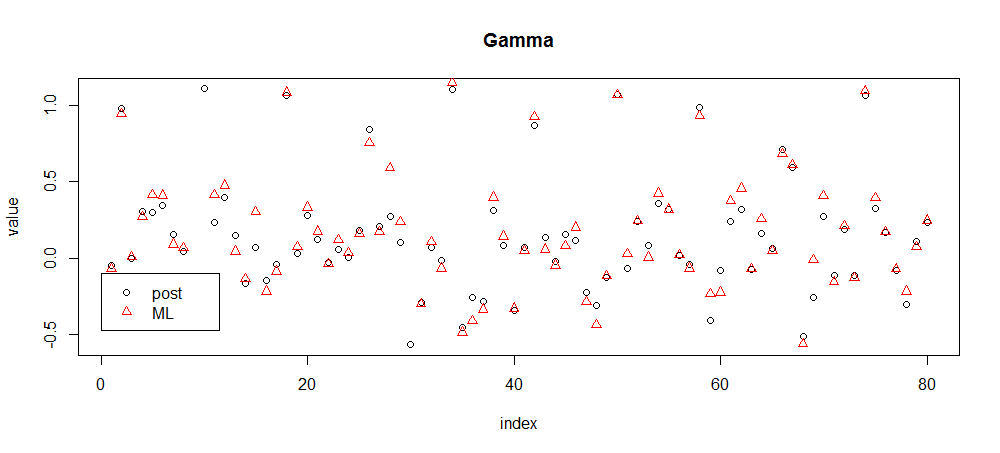
\includegraphics[width=15cm]{Pics/PlotGammaPostML.png}
	\caption{$\gamma$: posterior means vs. ML estimates}
\end{figure}
The posterior means are significantly updated in comparison with the priors but the values are in the same range.
\begin{figure}[!h]
	\centering
	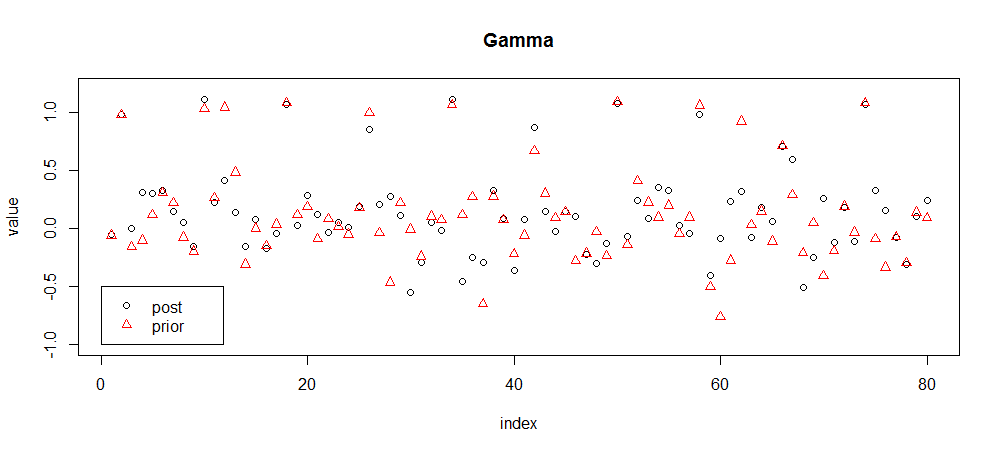
\includegraphics[width=15cm]{Pics/PlotGammaPostPrior.png}
	\caption{$\gamma$: posterior means vs. second stage prior means coming from the training sample}
\end{figure}
We can conclude that the draws of the parameter vector are reasonable. \\
Finally, compare the draws for the errors covariance matrix ($\Sigma$). Note that for Student-t distribution with 6 degrees of freedom the covariance matrix is a scaled version of the scale matrix $\Omega$: $\Sigma = \frac{\nu}{\nu - 2}\Omega = \frac{6}{4}\Omega$. We approximate the scale matrix $\Omega$ as the inverse of the posterior means of sample draws of $\Omega^{-1}$. 
\begin{figure}[!h]
	\centering
	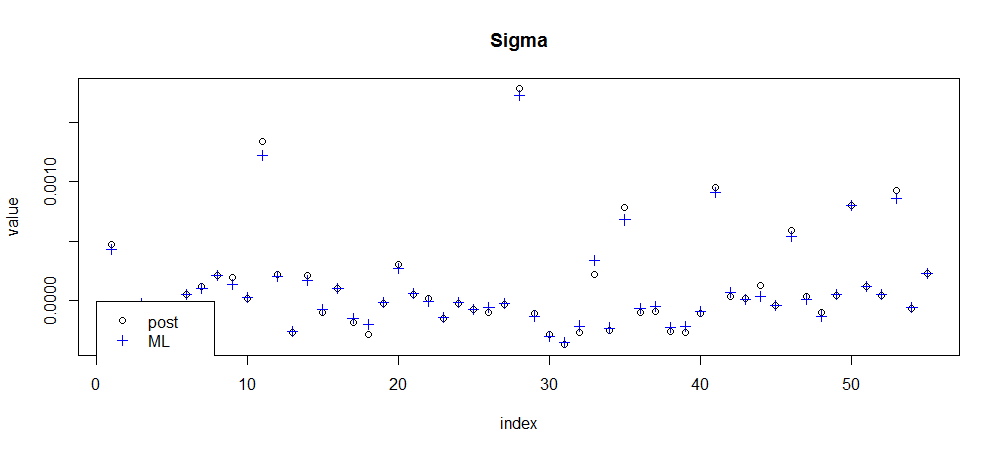
\includegraphics[width=15cm]{Pics/PlotSigmaPostML.png}
	\caption{$\Sigma$: posterior means vs. ML}
\end{figure}
\begin{figure}[!h]
	\centering
	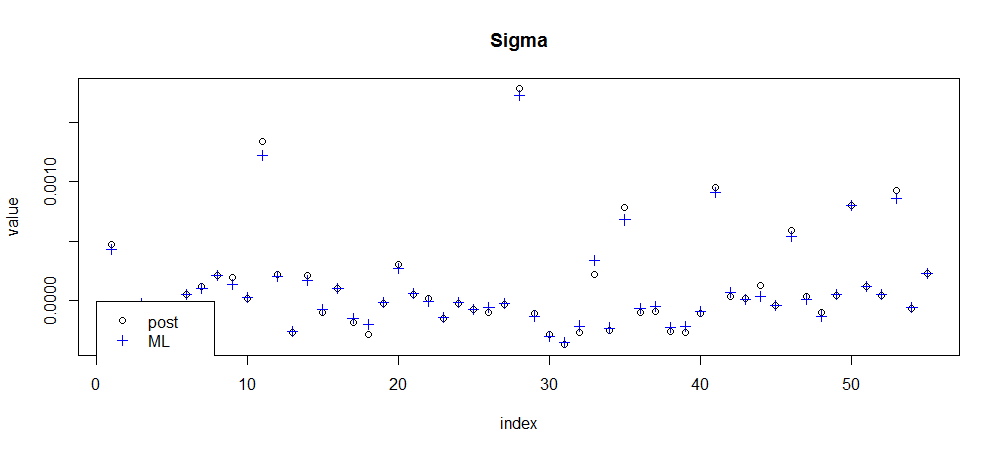
\includegraphics[width=15cm]{Pics/PlotSigmaPostML.png}
	\caption{$\Sigma$: posterior means vs. second stage prior means}
\end{figure}
Again, the results from two methods are similar, so we conclude that the procedure produces reasonable estimates of the parameters of interest.
\section{Change of Models}
\end{document}
